\documentclass{beamer}

\usepackage{amsmath, amssymb}
\usepackage{tikz-cd}
\usepackage{xcolor}
\usepackage{graphicx}

\title{MT222: Calculus II}
\author{\textbf{Miraj Samarakkody}}
\institute{Tougaloo College}
\date{03/26/2025}

\begin{document}

\begin{frame}
    \titlepage
\end{frame}




\begin{frame}{}
    \begin{center}
        \Huge{7.3 - Trigonometric Substitution}
    \end{center}
    
\end{frame}

\begin{frame}{Why we need this?}
    Think about finding the area under the curve of a semi-circle
\end{frame}

\begin{frame}{Table of Trigonometric Substitiution}
    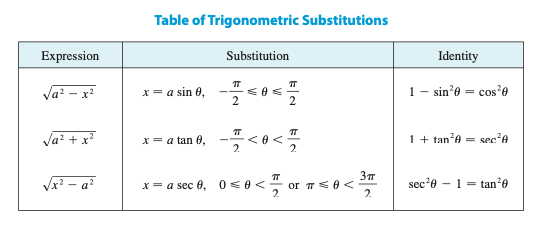
\includegraphics[scale=0.6]{figures/fig_1.png}
\end{frame}

\begin{frame}
    \frametitle{Example 1}
Evaluate \[\int \dfrac{\sqrt{9-x^2}}{x^2}~dx\]
\end{frame}

\begin{frame}{Example 2}
    Find the area enclosed by the ellipse \[\dfrac{x^2}{a^2}+ \dfrac{y^2}{b^2}=1\]
\end{frame}



\end{document}